%% file: example.tex = LaTeX + BibTex example for article-like report
%% init: sometime 1993 for my practical "Stellar Spectra A"
%% last: Jan 17 2020  Rob Rutten  Deil
%% site: http://www.staff.science.uu.nl/~rutte101/rrweb/rjr-edu/manuals/student-report/

%% First read ``latex-bibtex-simple-manual'' at
%% http://www.staff.science.uu.nl/~rutte101/Report_recipe.html

%% Then run this file to see what it does:
%%    latex example     bibtex example     latex example     latex example
%% inspect with xdvi example &, or pdflatex into example.pdf for inspection.

%% Take out my content to make a template for your report.

%%%%%%%%%%%%%%%%%%%%%%%%%%%%%%%%%%%%%%%%%%%%%%%%%%%%%%%%%%%%%%%%%%%%%%%%%%%%
\documentclass{aa-note}    %% Astronomy & Astrophysics style class aa.cls v8.2

%% load latex packages
\usepackage{graphicx,url,twoopt,natbib}
\usepackage[varg]{txfonts}           %% old-fashioned A&A font choice
\usepackage{hyperref}                %% for pdflatex
%%\usepackage[breaklinks]{hyperref}  %% for latex+dvips, not for pdflatex
%%\usepackage{breakurl}              %% for latex+dvips, not for pdflatex

%% define link colors
\hypersetup{
  colorlinks=true,   %% links colored instead of frames
  urlcolor=blue,     %% external hyperlinks
  linkcolor=blue     %% internal latex links (eg Fig)
}

\usepackage{float} 
\usepackage{subfigure} 

\bibpunct{(}{)}{;}{a}{}{,}    %% natbib cite format used by A&A and ApJ
\pagestyle{plain}             %% undo the fancy A&A pagestyle
\let\footnotesize\tiny        %% keep this to 1 page (aa.cls sets \small)

%% Add commands to add a note or link to a reference
\makeatletter
\newcommand{\bibnote}[2]{\global\@namedef{#1note}{#2}}
\newcommand{\biblink}[2]{\global\@namedef{#1link}{#2}}
\makeatother

%% Commands to make citations ADS clickers and to add such also to refs.
%% The twoopt definition permits parameters as in natbib (which I never use).
%% The stonyslink solves a stop problem when using latex instead of pdflatex.
%% May 20 2019: switch to "new" ADS (classic in EDP/A&A readme still work)
\makeatletter
  \protected\def\stonyslink{%
     \def\hyper@linkstart##1##2{}\let\hyper@linkend\@empty}
  \newcommandtwoopt{\citeads}[3][][]{%
   \href{http://ui.adsabs.harvard.edu/abs/#3/abstract}%
        {\stonyslink \citealp[#1][#2]{#3}}%   %% Rutten, 2000
   \biblink{#3}{\href{http://ui.adsabs.harvard.edu/abs/#3/abstract}{ADS}}}
 \newcommandtwoopt{\citepads}[3][][]{%
   \href{http://ui.adsabs.harvard.edu/abs/#3/abstract}%
        {\stonyslink \citep[#1][#2]{#3}}%     %% (Rutten 2000)
   \biblink{#3}{\href{http://ui.adsabs.harvard.edu/abs/#3/abstract}{ADS}}}
 \newcommandtwoopt{\citetads}[3][][]{%
   \href{http://ui.adsabs.harvard.edu/abs/#3/abstract}%
        {\stonyslink \citet[#1][#2]{#3}}%     %% Rutten (2000)
  \biblink{#3}{\href{http://ui.adsabs.harvard.edu/abs/#3/abstract}{ADS}}}
 \newcommandtwoopt{\citeyearads}[3][][]{%
   \href{http://ui.adsabs.harvard.edu/abs/#3/abstract}%
        {\stonyslink \citeyear[#1][#2]{#3}}%  %% 2000
   \biblink{#3}{\href{http://ui.adsabs.harvard.edu/abs/#3/abstract}{ADS}}}
\makeatother

%% ADS specific page opener = {bibcode}{pdf page number}{link text}.
%% ADS promised that the "classic" link below keeps working in "new" ADS;
%% I use it because it opens ADS bibcode pdf's and ADS arXiv altcode pdf's
%% whereas "new" ADS needs separate commands (to PUB_PDF and EPRINT_PDF)
\def\linkadspage#1#2#3{\href{http://adsabs.harvard.edu/cgi-bin/nph-data_query?bibcode=#1\&link_type=ARTICLE\&db_key=AST\#page=#2}{#3}}

%% Spectral species
\def\HI{\ion{H}{I}}            %% A&A; for aastex use \def\HI{\ion{H}{1}}
\def\MgI{\ion{Mg}{I}}          %% A&A; for aastex use \def\MgI{\ion{Mg}{1}}
\def\MgII{\ion{Mg}{II}}        %% A&A; for aastex use \def\MgII{\ion{Mg}{2}}

%% Hyphenation
\hyphenation{Schrij-ver}       %% Dutch ij is a single character


%%%%%%%%%%%%%%%%%%%%%%%%%%%%%%%%%%%%%%%%%%%%%%%%%%%%%%%%%%%%%%%%%%%%%%%%%%%%
\begin{document}

%% Simple header (replacing A&A commands which produce the A&A banner)

\twocolumn[{%
\vspace*{4ex}
\begin{center}
  {\Large \bf Impact of number of steps used to generate the time series on the results}\\[4ex]
  {\large \bf Niu Liu
%  $^{1}$
  % , S\'{e}bastien Lambert. Carlsson$^2$
              % and N. G. Shchukina$^3$
              }\\[4ex]
%  \begin{minipage}[t]{16cm} \small
%        $^1$ School of Astronomy and Space Science,
%        Key Laboratory of Modern Astronomy and Astrophysics (Ministry of Education),
%        Nanjing University, Nanjing, P. R. China\\
%        % $^2$ SYRTE, Observatoire de Paris, Universit\'{e} PSL, CNRS,
%        % Sorbonne Universit\'{e}, LNE, Paris, France\\
%        % $^3$ Main Astronomical Observatory,
%        %      252127 Kiev, Ukraine\\
%
%%  {\bf Abstract.~}
%   \vspace*{2ex}
%  \end{minipage}
\end{center}
}]


%%%%%%%%%%%%%%%%%%%%%%%%%%%%%%%%%%%%%%%%%%%%%%%%%%%%%%%%%%%%%%%%%%%%%%%%%%%%
\section{Introduction}     \label{sec:introduction}
%%%%%%%%%%%%%%%%%%%%%%%%%%%%%%%%%%%%%%%%%%%%%%%%%%%%%%%%%%%%%%%%%%%%%%%%%%%%

In this note, I study how the number of steps used to generate the global time series affects the assessment of the ICRF3 axis stability.
I ran separately a 4-, 8-, 10-, and 20-step solution. 
Then on the one hand, I estimated the apparent proper motion for extragalactic sources and fitted the global spin of the CRF axis (Sect.~\ref{sec:spin}).
On the other hand, I computed the annual mean positions of sources to construct the yearly CRF and estimated their relative rotation and glide wrt. the ICRF3 S/X-band frame (Sect.~\ref{sec:yearly-crf}).
Some things that may lead to confusions are pointed out here.
In some plots, I used $\omega_x$, $\omega_y$, and $\omega_z$, while in others I used $\omega_1$, $\omega_2$, and $\omega_3$.
In fact, they refer to the same things.
It is the same for the $g$ parameter.
Another thing is that I used words ``rotation'' and ``glide'' in the title of some figures, but they are not always referred to the same things.
Sometimes, the rotation and glide parameters were estimated from the proper motion data, whilst they can also be estimated from the positional offset.
I did not spell it out clearly when I made these plots, but you may find the exact information from the captions. 
They can also be told from the unit.

%estimation of the global spin of the CRF axis. 
%I ran separately a 4-, 8-, 10-, and 20-step solution.  


%%%%%%%%%%%%%%%%%%%%%%%%%%%%%%%%%%%%%%%%%%%%%%%%%%%%%%%%%%%%%%%%%%%%%%%%%%%%
\section{Proper motion and derived spin}     \label{sec:spin}
%%%%%%%%%%%%%%%%%%%%%%%%%%%%%%%%%%%%%%%%%%%%%%%%%%%%%%%%%%%%%%%%%%%%%%%%%%%%

First, I considered only the subset of the ICRF3 defining sources, as shown in Fig. \ref{fig:spin-def}. 
For different number of steps, the spin and glide are fully consistent with the error bar. 
The rotation and glide axis is about 80 deg and 40 deg away from the GC. 
I think that we cannot make any firm conclusion on relationship between the estimated spin and glide vectors and the GA effect.

Second, I considered all the sources with a determinable apparent proper motion and used the bootstrap sampling technique to estimate the mean spin and glide. 
For a given sample size $N$, I randomly picked $N$ sources from the sample to form a subset and estimated the glide and spin based on this subset. 
This procedure was repeated 1000 times.
The mean value and standard deviation of the spin and glide parameters were used as the estimations of mean spin and glide and their uncertainties.
The sample size varied from 100 to 1000 with a step of 100.
The results are presented in Fig.~\ref{fig:spin-glide-all}.
The noticeable difference occurs to $\omega_z$ (or $\omega_3$, they are the same thing.) and $g_z$ (or $g_3$), which become insignificant when the number of step increases.

I took the weighted mean values of glide and rotation parameters in Fig.~\ref{fig:spin-glide-all} as the mean spin and glide.
The results are shown in Fig.~\ref{fig:spin-all}. 
We can found that the spin around the Z-axis ($\omega_3$ or $\omega_z$) decreases if using more than four steps. 
Similarly, the glide parameters ($g_1$ and $g_3$, or $g_x$ and $g_z$) also decreases. 
The glide axis is far from the GC direction, however, the rotation axis direction is very close to that of GC. 


%% {fig:waterfalls}
%===========================================================================
 \begin{figure*}%[hbtp]
   \centering
   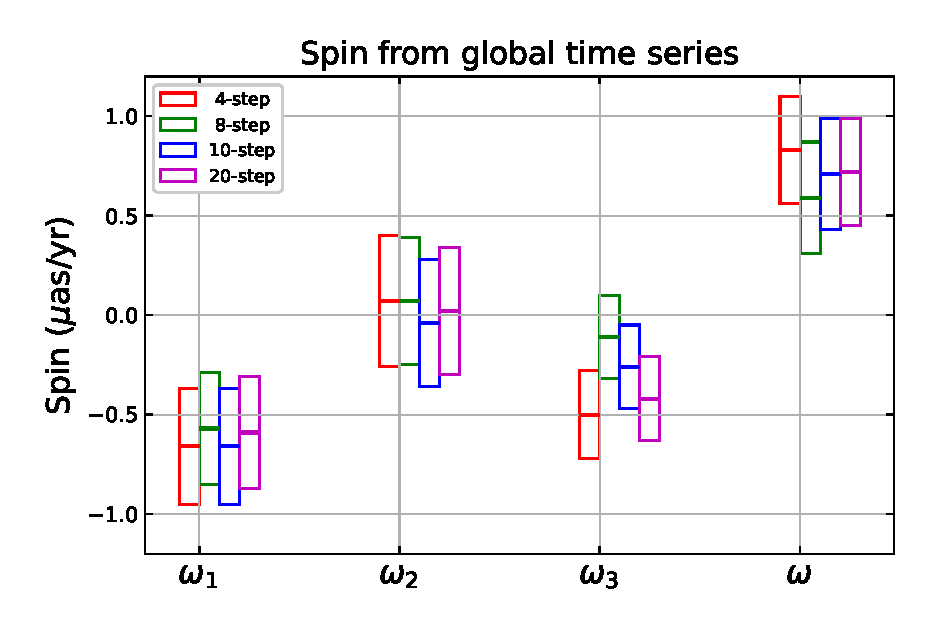
\includegraphics[width=80mm]{figs/spin-vs-nb-step-def} 
   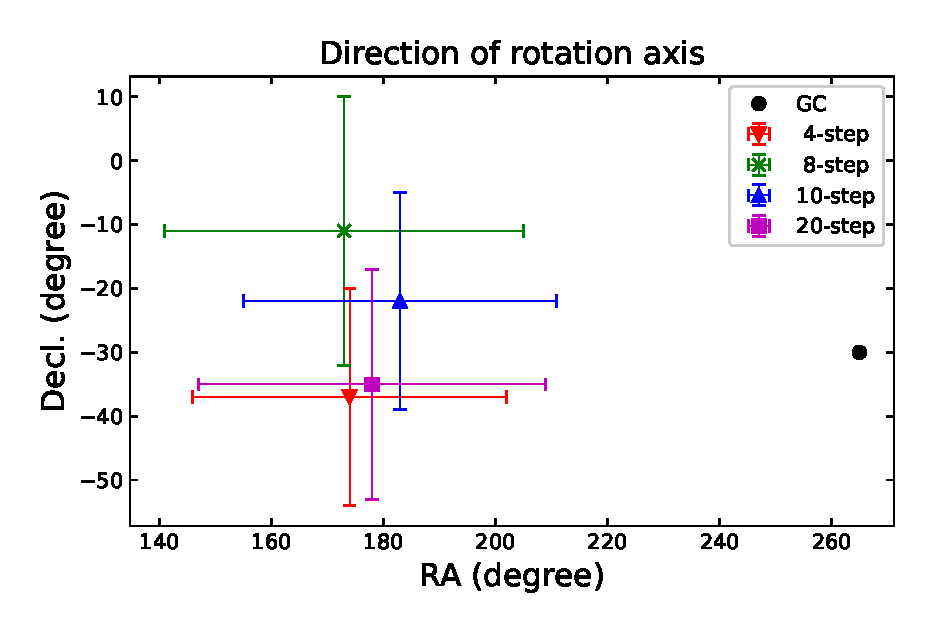
\includegraphics[width=80mm]{figs/spin-axis-vs-nb-step-def} \\
   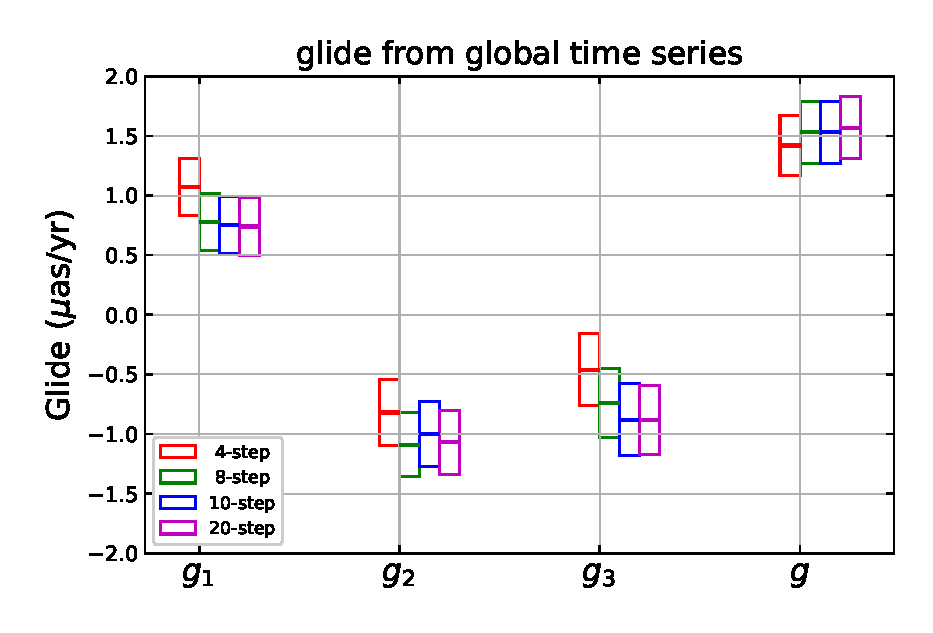
\includegraphics[width=80mm]{figs/glide-vs-nb-step-def} 
   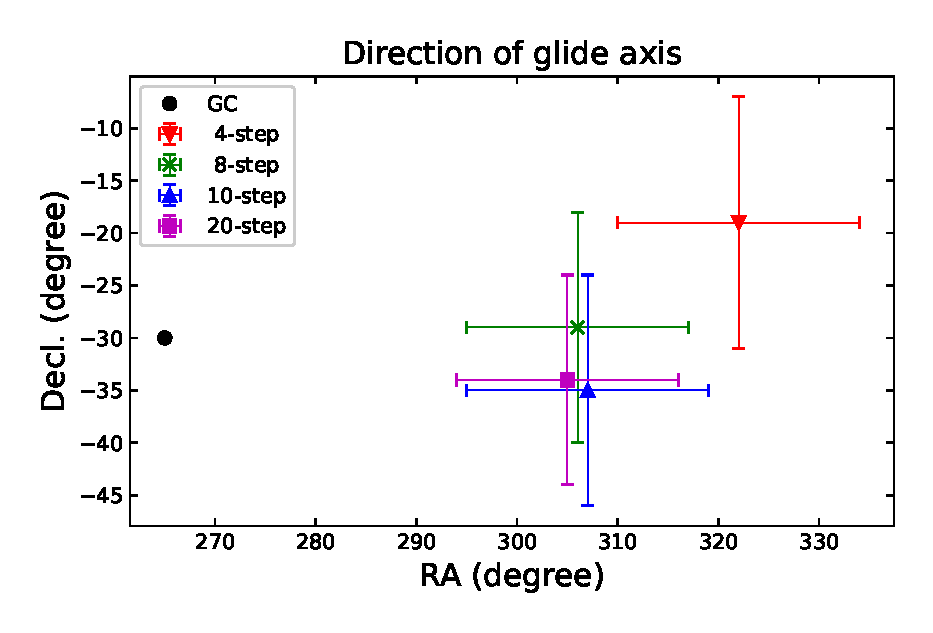
\includegraphics[width=80mm]{figs/glide-axis-vs-nb-step-def}  
   \caption[]{\label{fig:spin-def} %
   Rotation and glide parameters from the apparent proper motions of the subset of ICRF3 defining sources.
   }
 \end{figure*}
% ===========================================================================
%% Have "floats" such as figures between blank lines to make them float

%% {fig:waterfalls}
%===========================================================================
 \begin{figure*}%[hbtp]
   \centering
   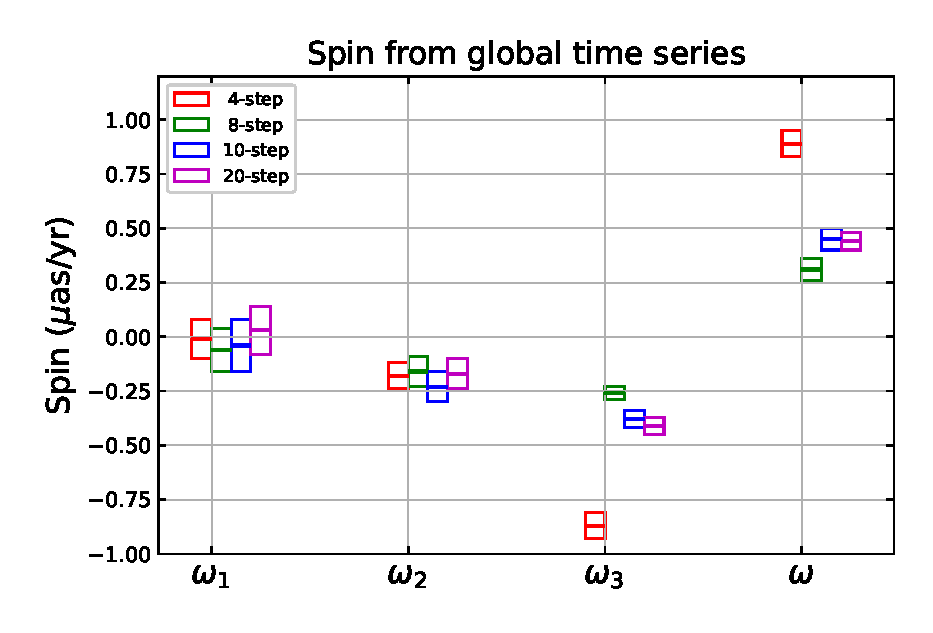
\includegraphics[width=80mm]{figs/spin-vs-nb-step-all} 
   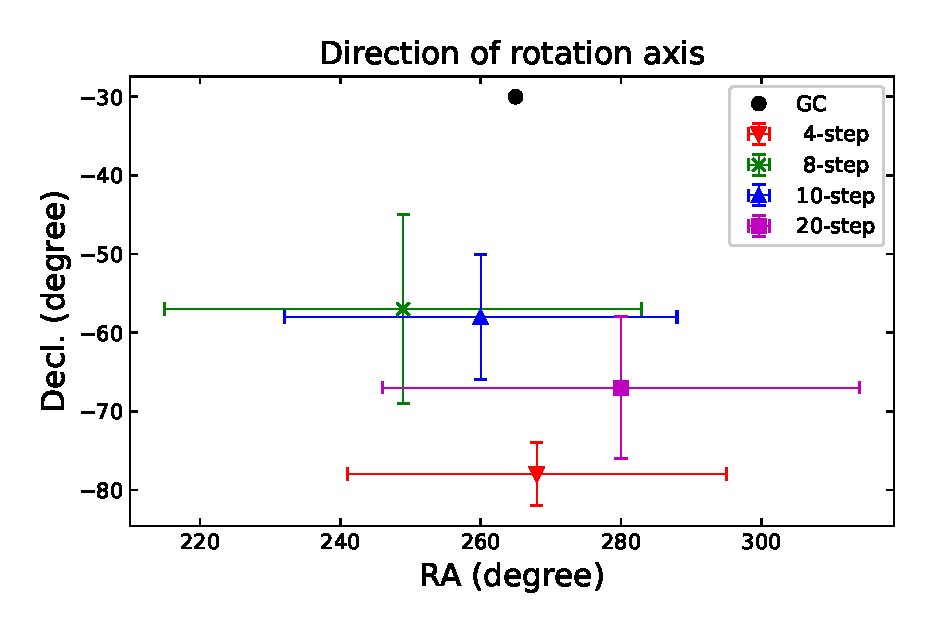
\includegraphics[width=80mm]{figs/spin-axis-vs-nb-step-all} \\
   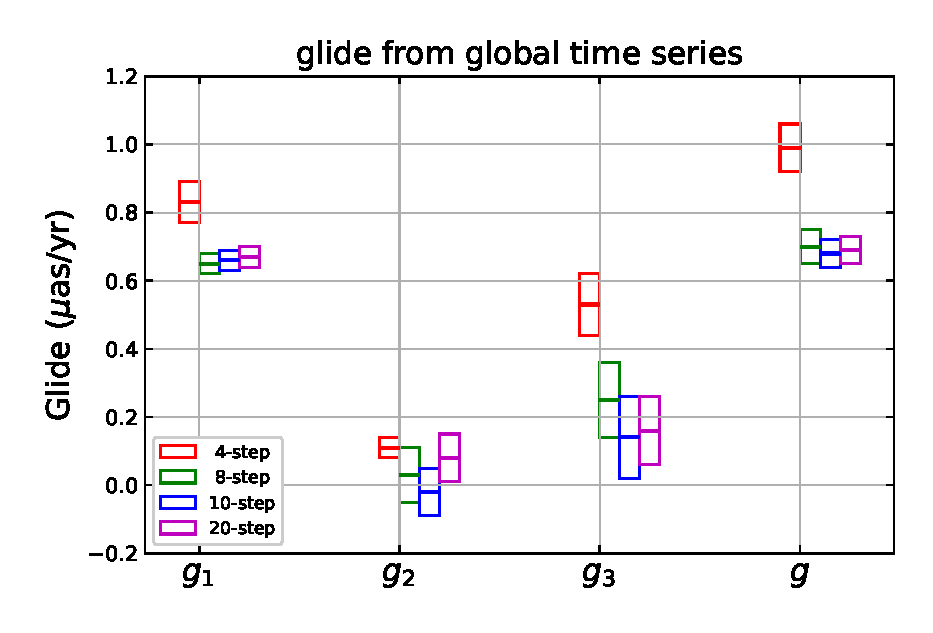
\includegraphics[width=80mm]{figs/glide-vs-nb-step-all} 
   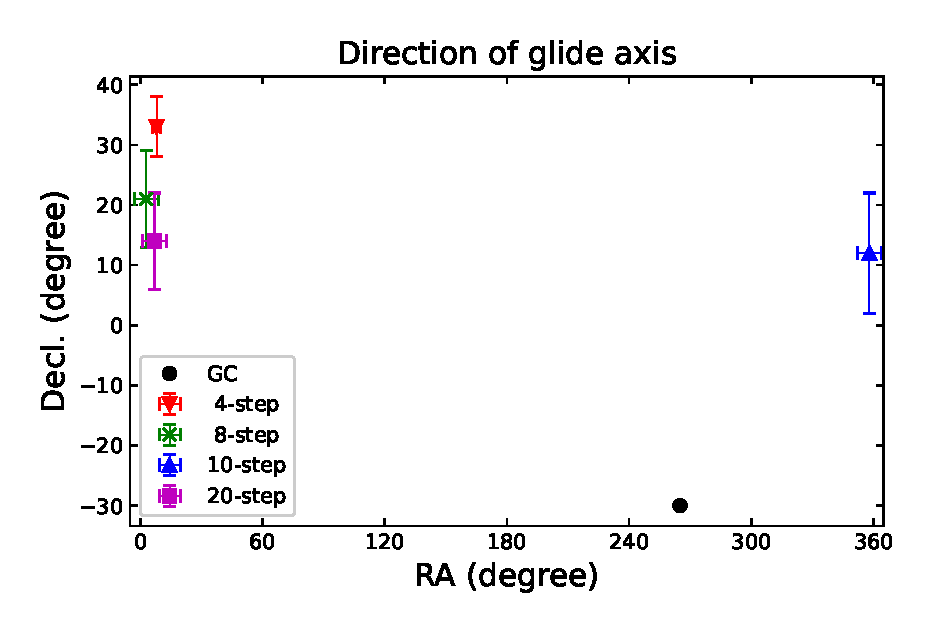
\includegraphics[width=80mm]{figs/glide-axis-vs-nb-step-all}  
   \caption[]{\label{fig:spin-all} %
   Rotation and glide parameters from the apparent proper motions of the subset of sources with a determinable apparent proper motion, i.e., number of time series data points $\ge$ 5.
   }
 \end{figure*}
% ===========================================================================
%% Have "floats" such as figures between blank lines to make them float

 \begin{figure*}[hbtp]
   \centering
   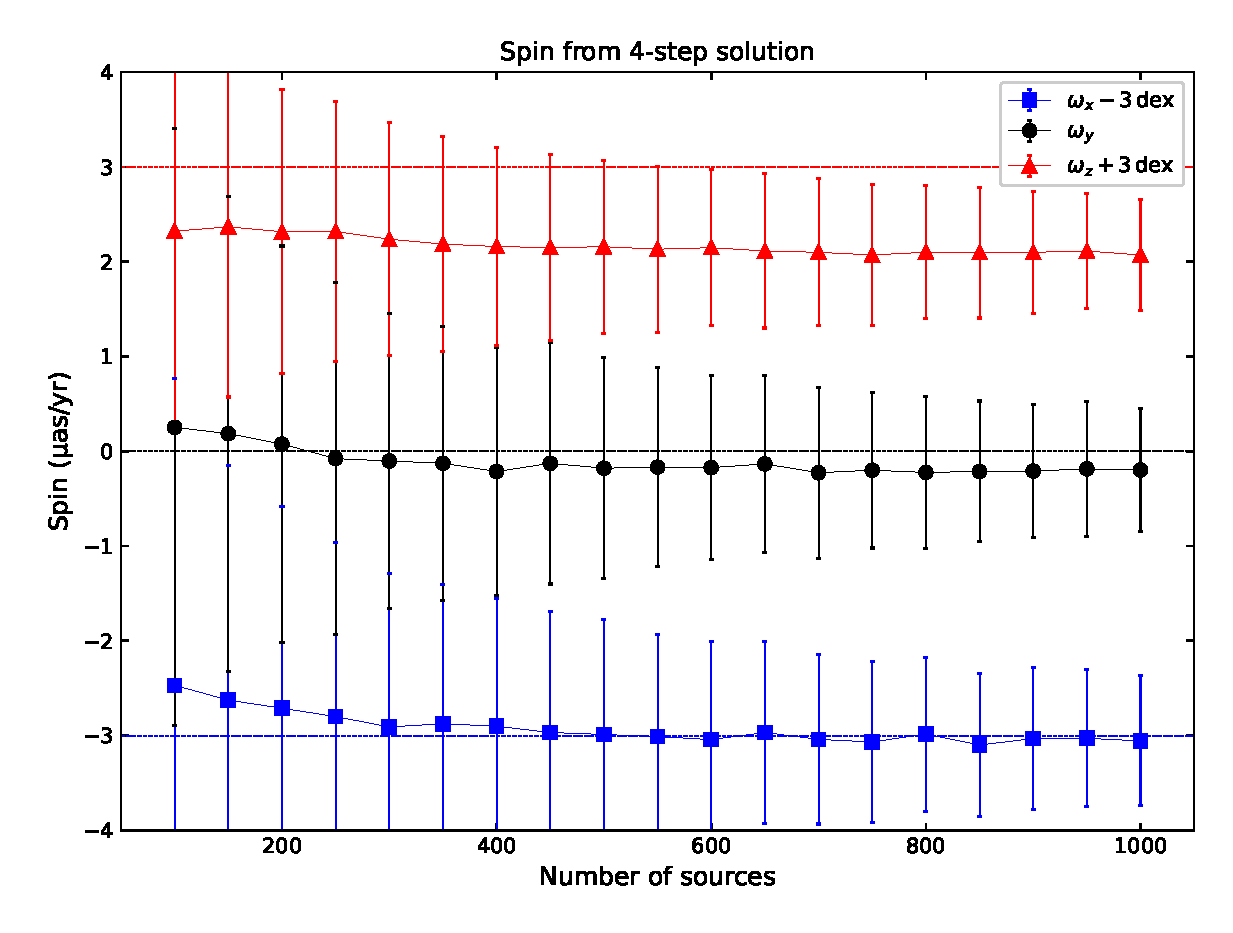
\includegraphics[width=80mm]{figs/spin-from-apm-nju-4step} 
   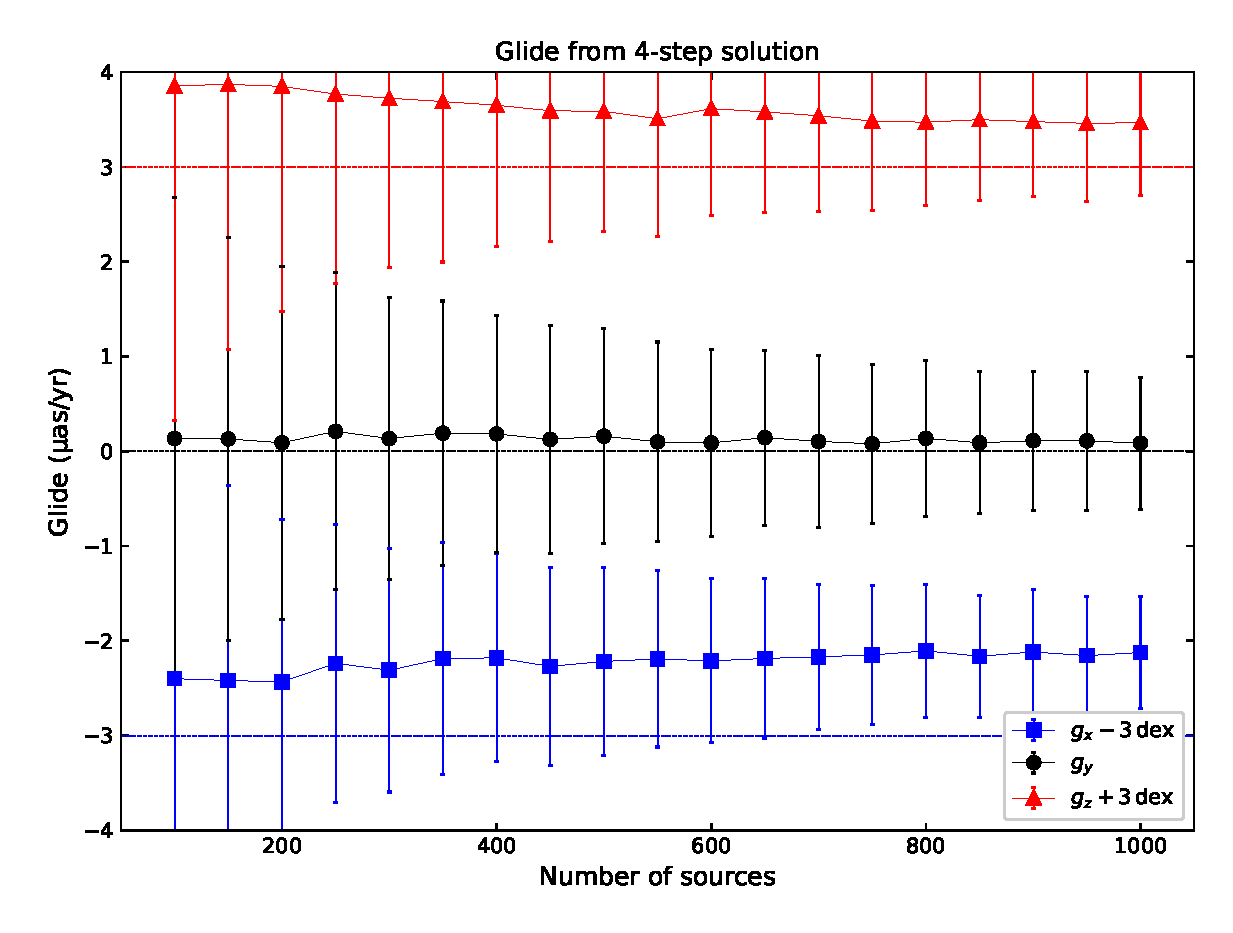
\includegraphics[width=80mm]{figs/glide-from-apm-nju-4step} \\
   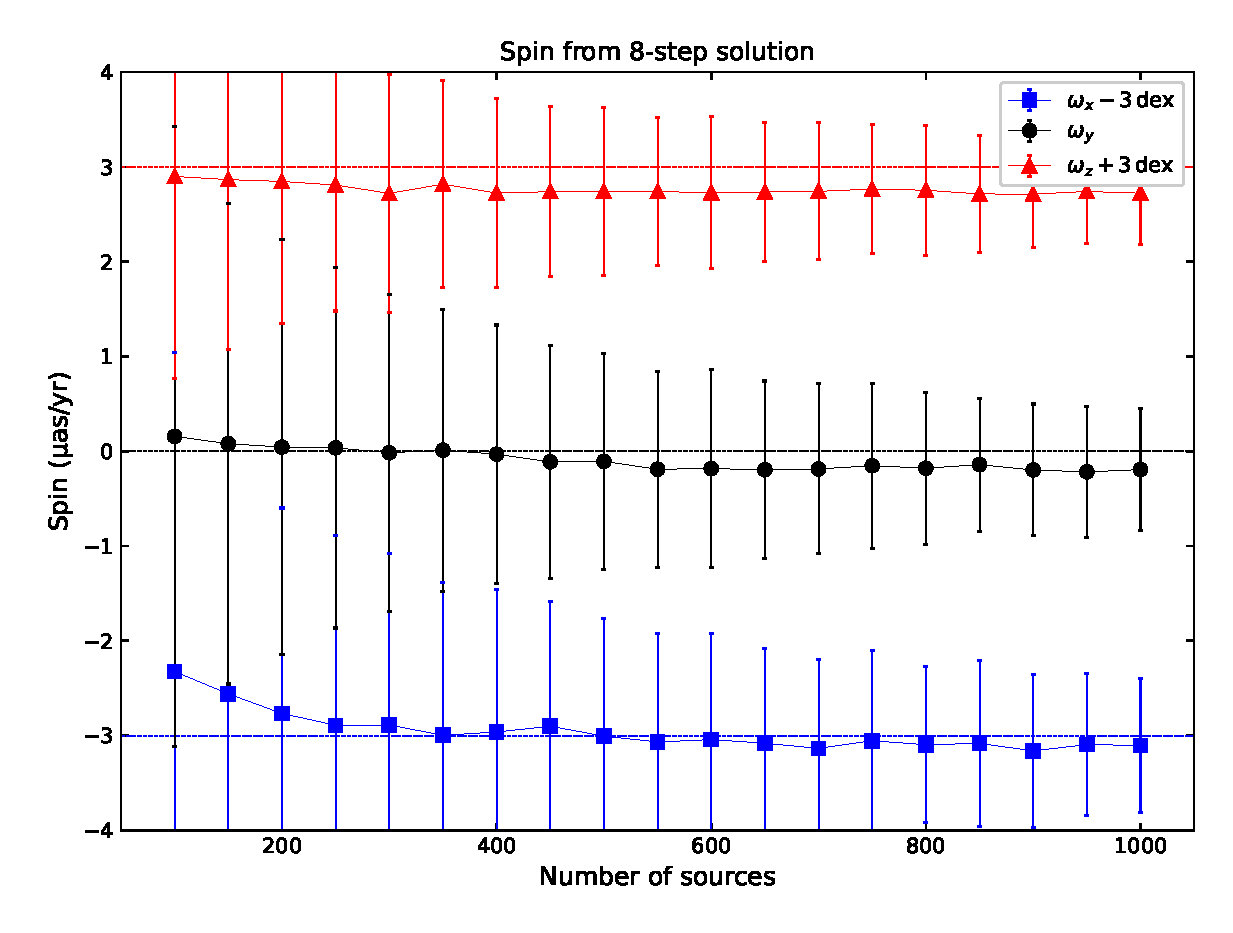
\includegraphics[width=80mm]{figs/spin-from-apm-nju-8step} 
   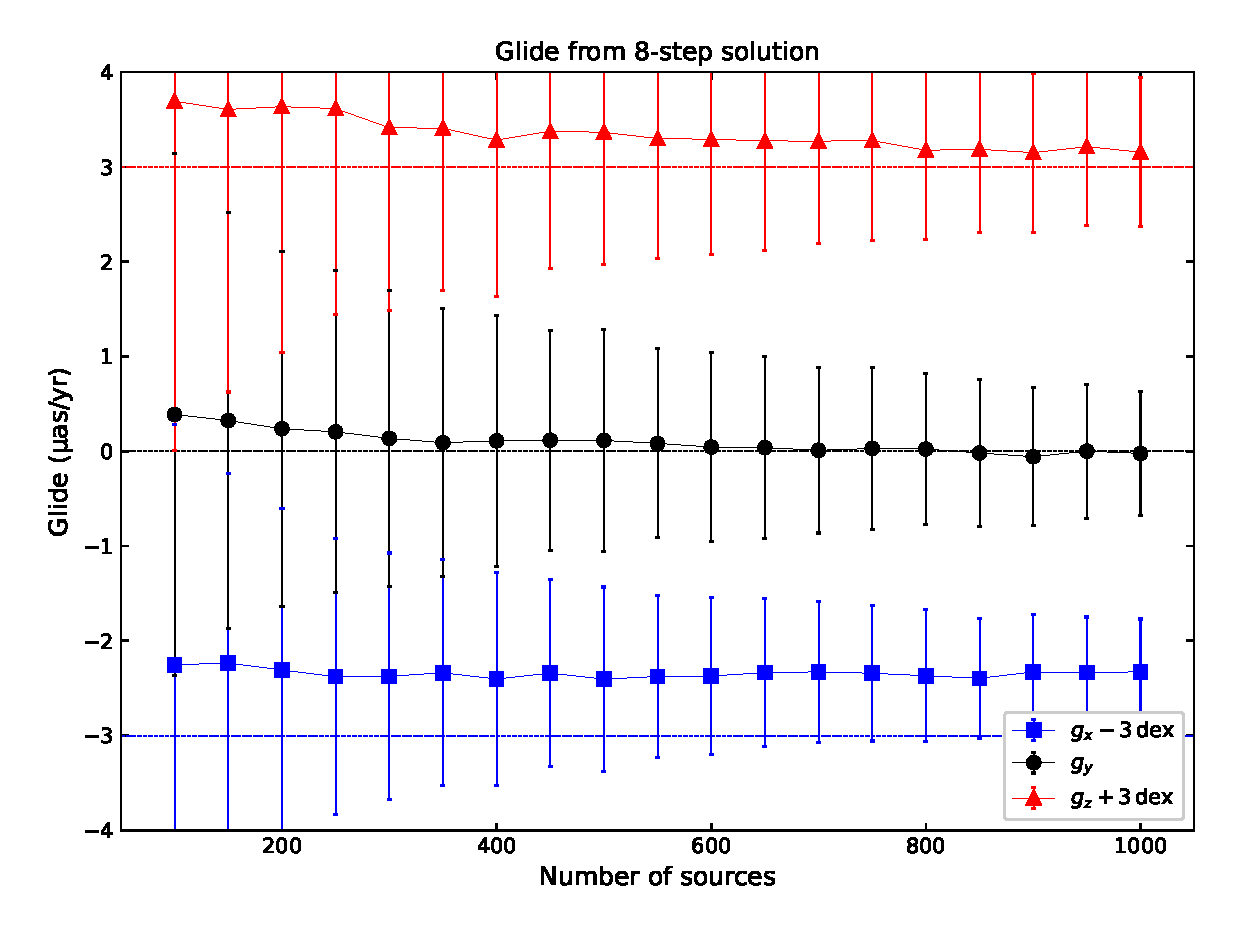
\includegraphics[width=80mm]{figs/glide-from-apm-nju-8step} \\
   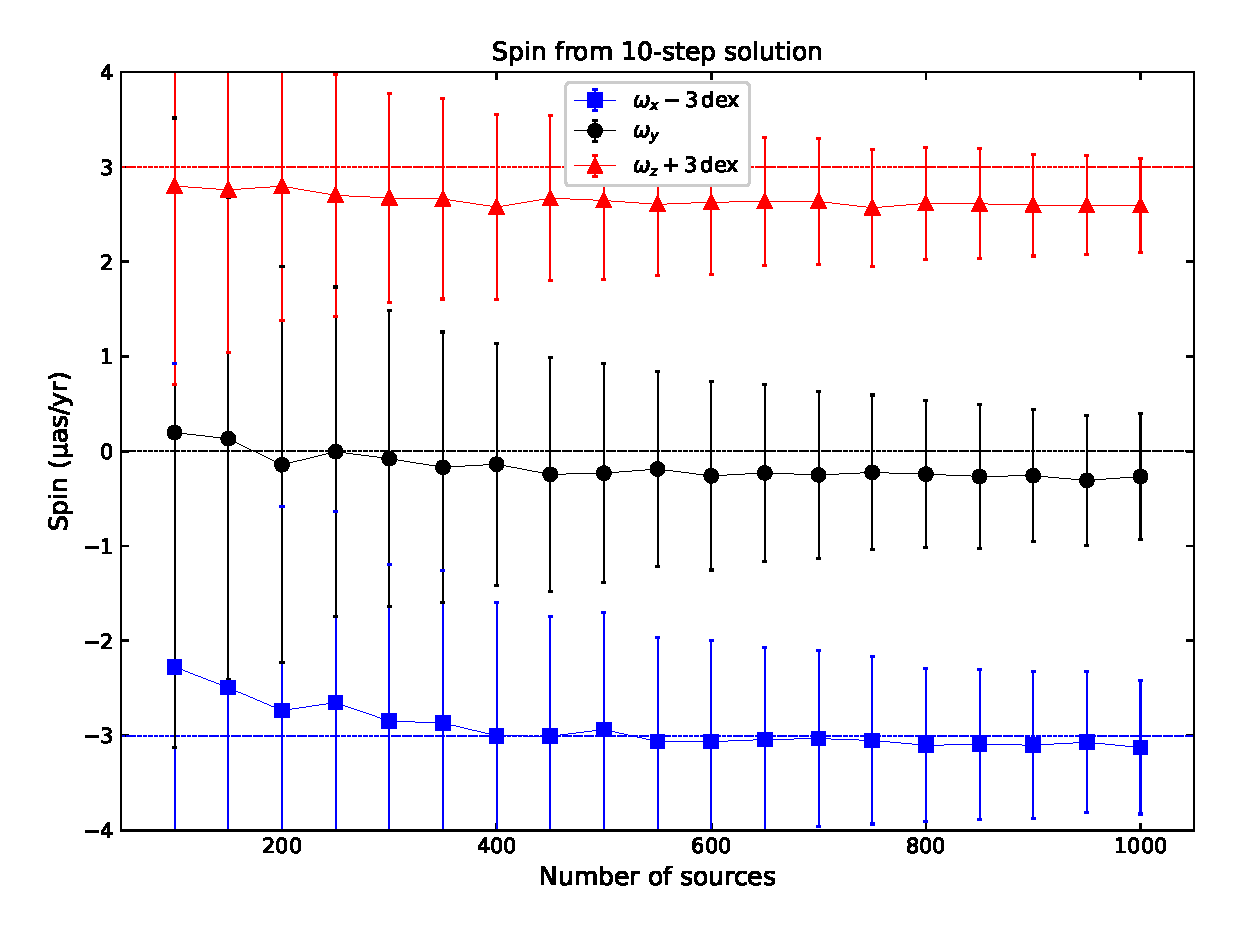
\includegraphics[width=80mm]{figs/spin-from-apm-nju-10step} 
   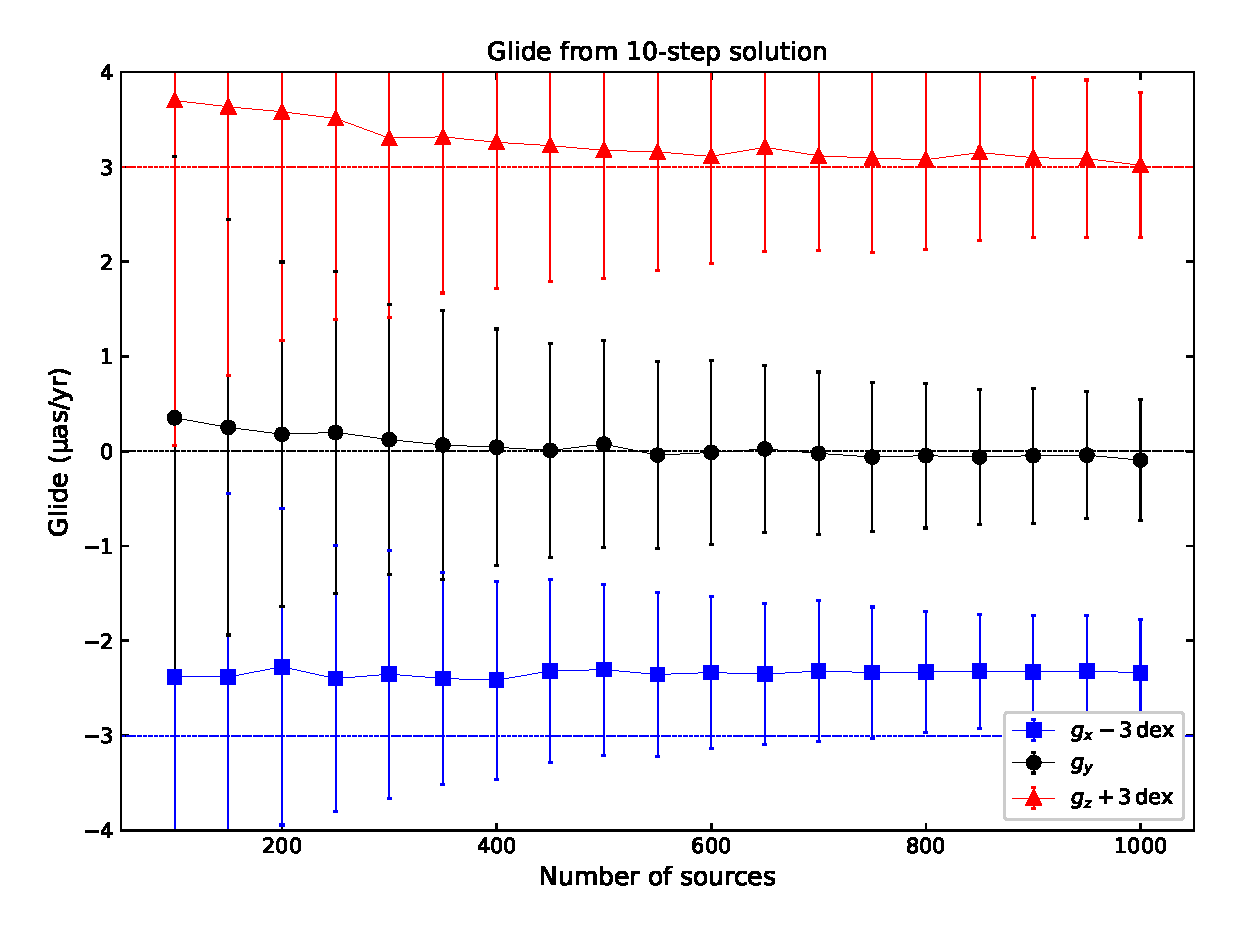
\includegraphics[width=80mm]{figs/glide-from-apm-nju-10step} \\
   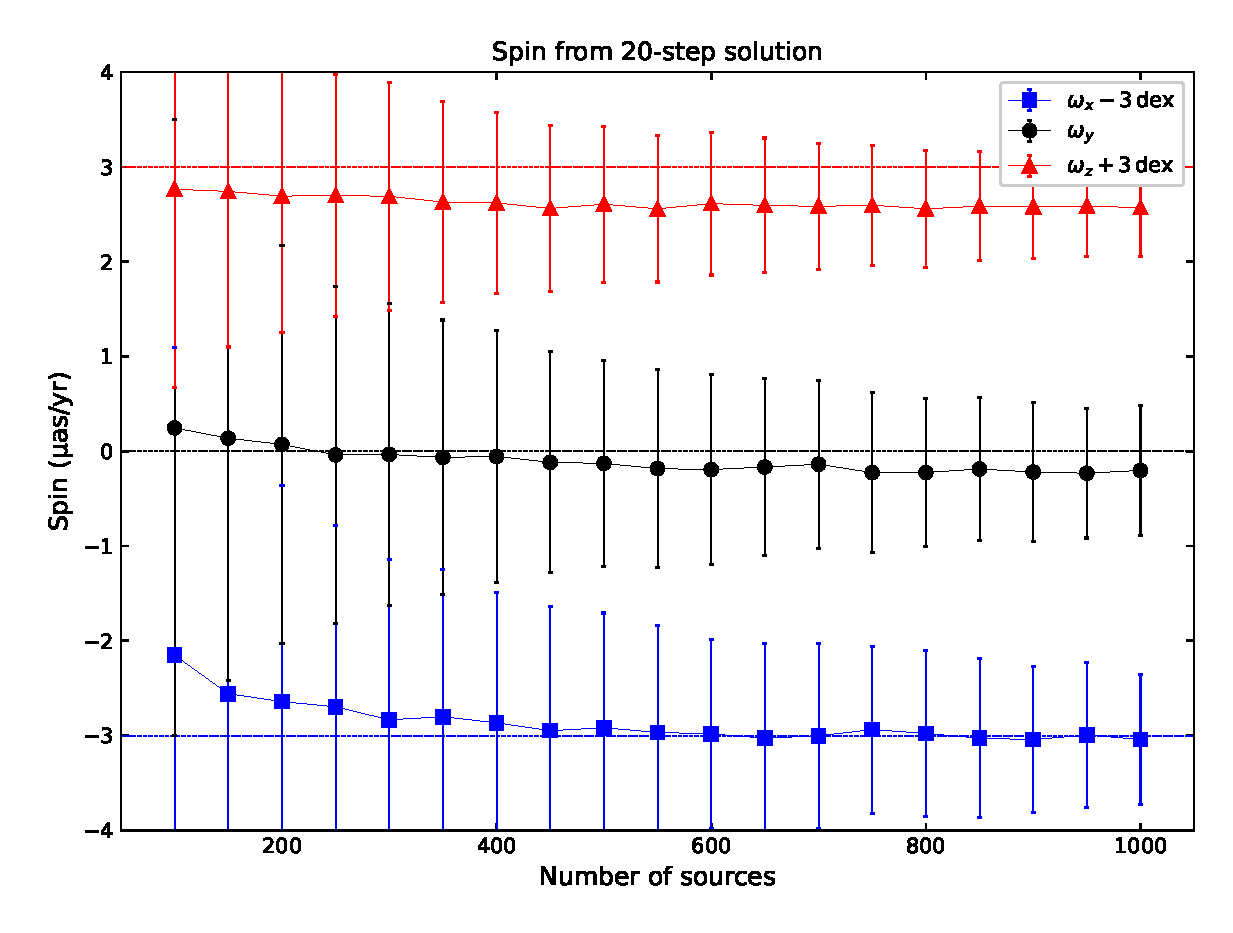
\includegraphics[width=80mm]{figs/spin-from-apm-nju-20step} 
   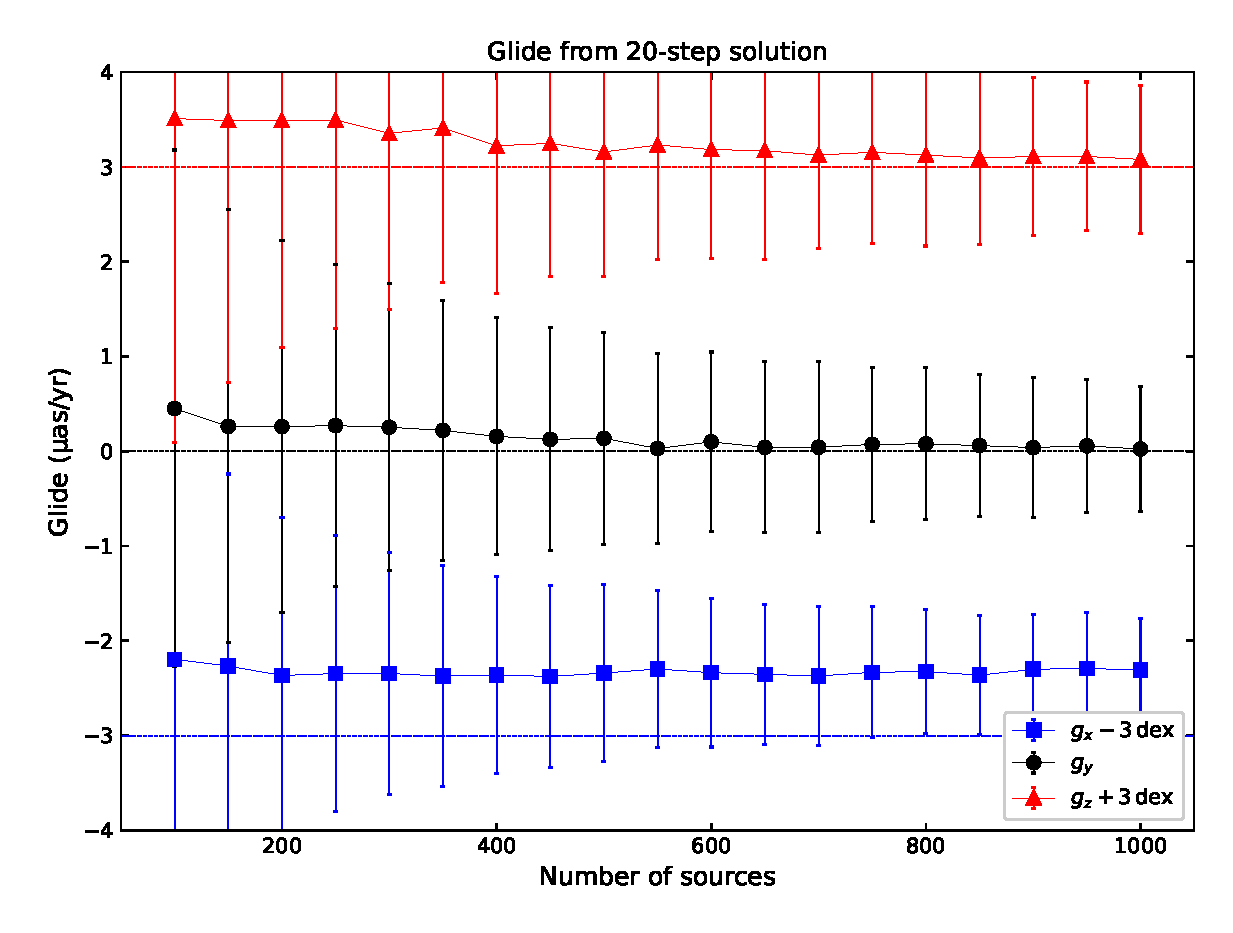
\includegraphics[width=80mm]{figs/glide-from-apm-nju-20step}
   \caption[]{\label{fig:spin-glide-all} %
   Rotation and glide parameters as a function of the sample size.
   These parameters are estimated from the apparent proper motions of sources with a determinable apparent proper motion, i.e., number of time series data points $\ge$ 5.
   }
 \end{figure*}
% ===========================================================================
%% Have "floats" such as figures between blank lines to make them float

%%%%%%%%%%%%%%%%%%%%%%%%%%%%%%%%%%%%%%%%%%%%%%%%%%%%%%%%%%%%%%%%%%%%%%%%%%%%
\section{Orientation of yearly CRF} \label{sec:yearly-crf}
%%%%%%%%%%%%%%%%%%%%%%%%%%%%%%%%%%%%%%%%%%%%%%%%%%%%%%%%%%%%%%%%%%%%%%%%%%%%


Figures~\ref{fig:rotation-plot} and \ref{fig:glide-plot} present the relative rotation and glide parameters of yearly CRFs with respective to the ICRF3 $S/X$-band catalog.
Only the ICRF3 defining sources were used.
I found that the influence of different choices of the number of steps on estimations of these parameters is rather tiny.

%% {fig:waterfalls}
%===========================================================================
 \begin{figure*}[hbtp]
   \centering
   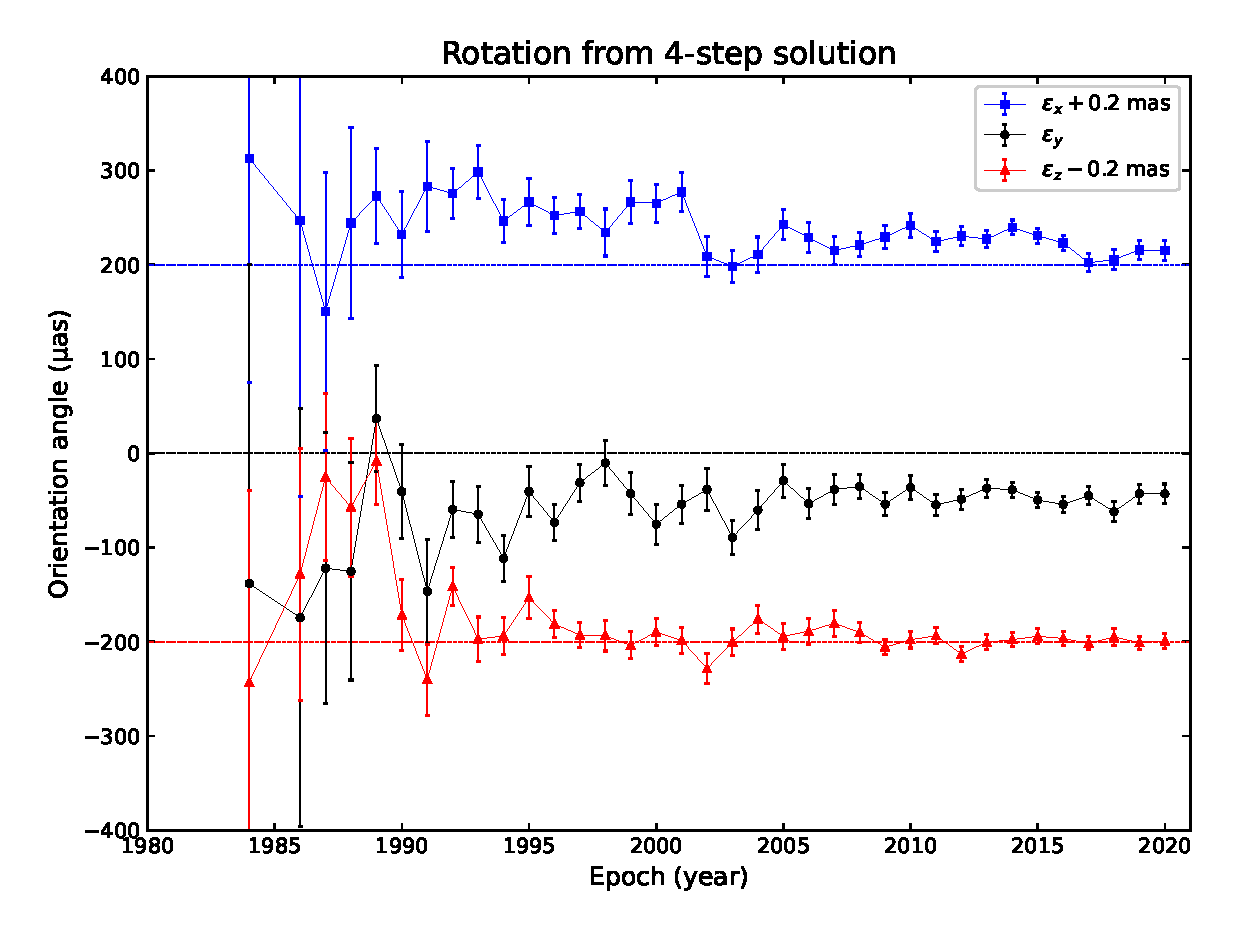
\includegraphics[width=75mm]{figs/orient-from-yearly-ts-nju} 
   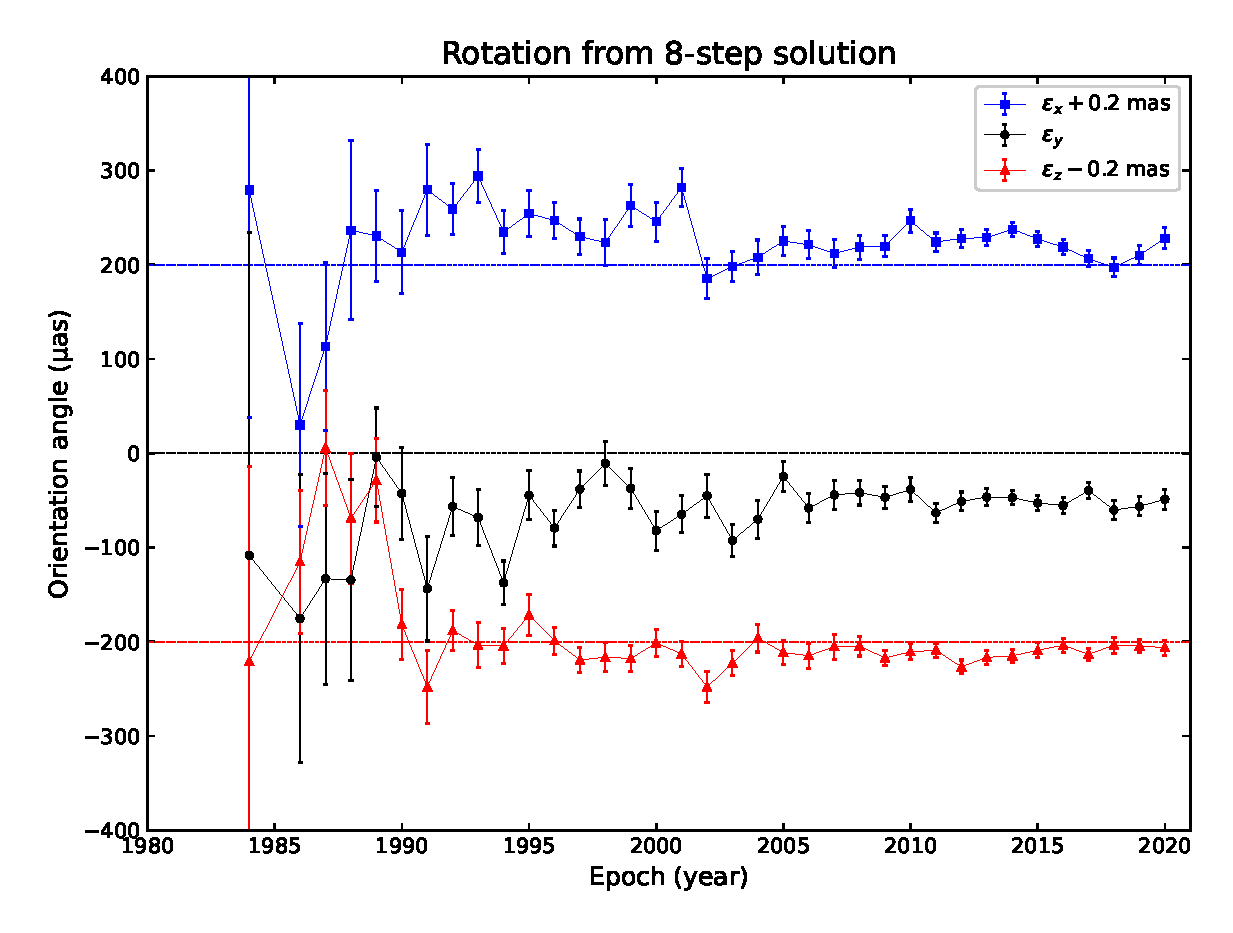
\includegraphics[width=75mm]{figs/orient-from-yearly-ts-nju-8step} \\
   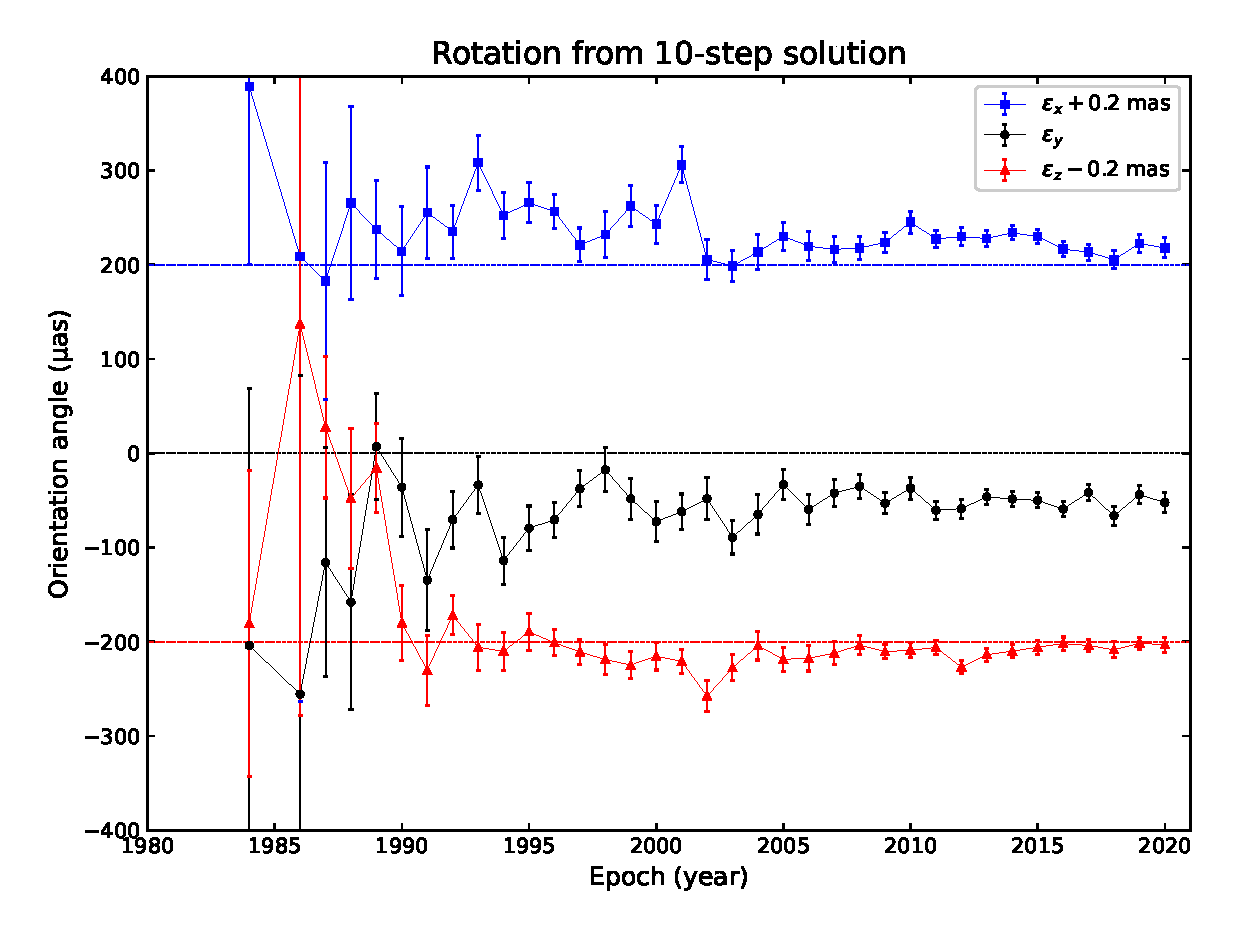
\includegraphics[width=75mm]{figs/orient-from-yearly-ts-nju-10step} 
   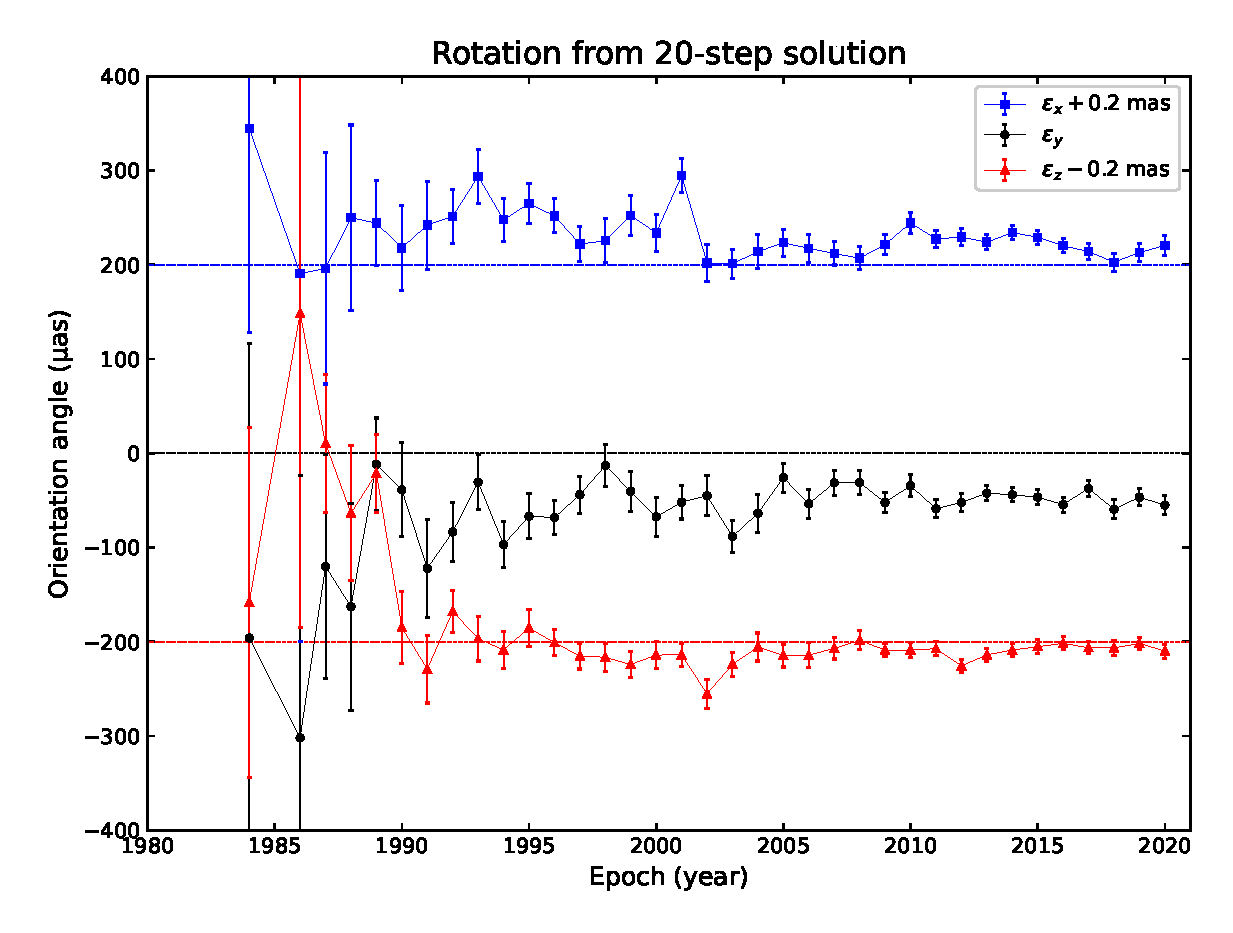
\includegraphics[width=75mm]{figs/orient-from-yearly-ts-nju-20step}  
   \caption[]{\label{fig:rotation-plot} %
   Rotation parameters of the yearly CRFs wrt. the ICRF3 S/X-band frame based on the ICRF3 defining sources.
   }
 \end{figure*}
% ===========================================================================
%% Have "floats" such as figures between blank lines to make them float

%% {fig:waterfalls}
%===========================================================================
 \begin{figure*}[hbtp]
   \centering
   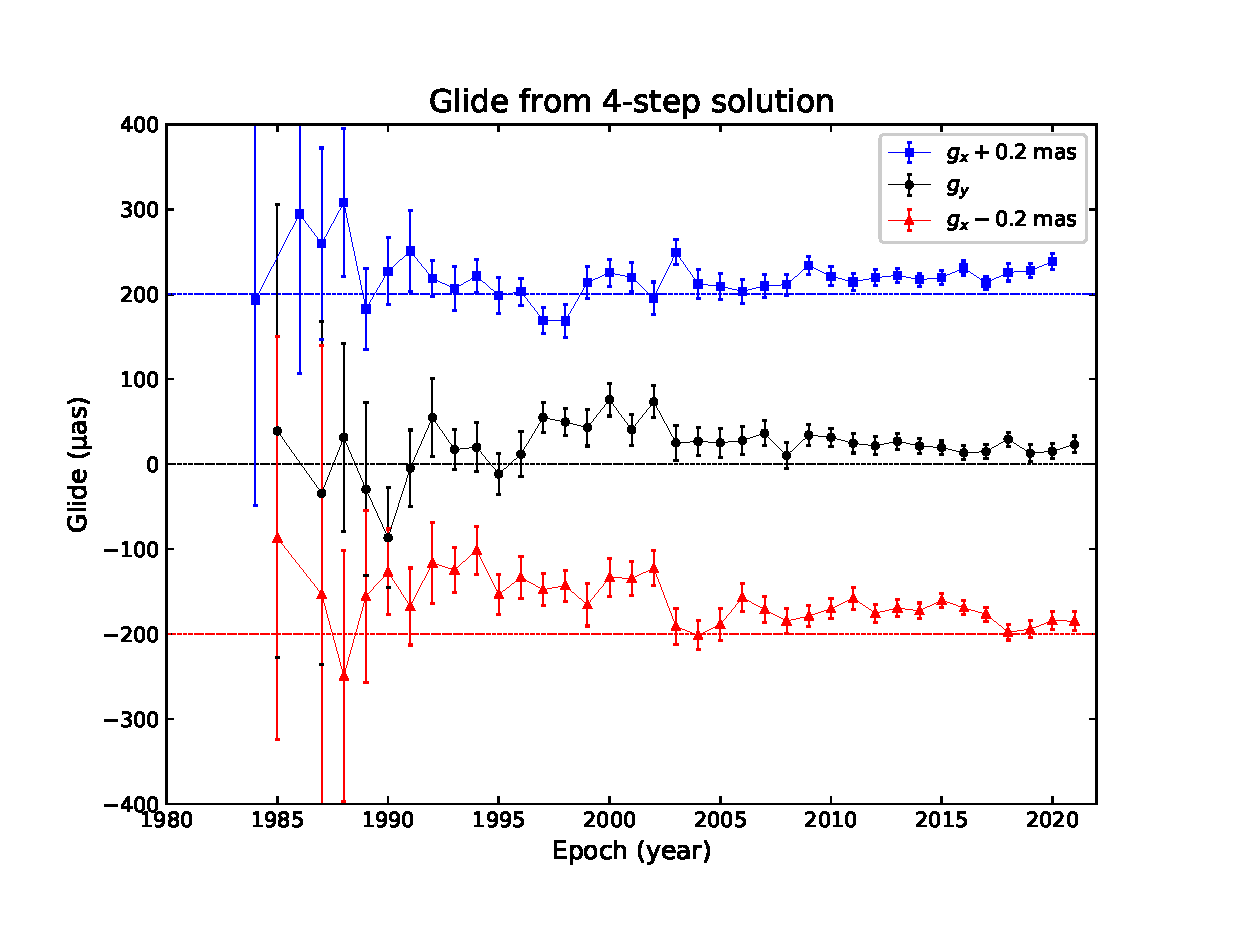
\includegraphics[width=75mm]{figs/glide-from-yearly-ts-nju} 
   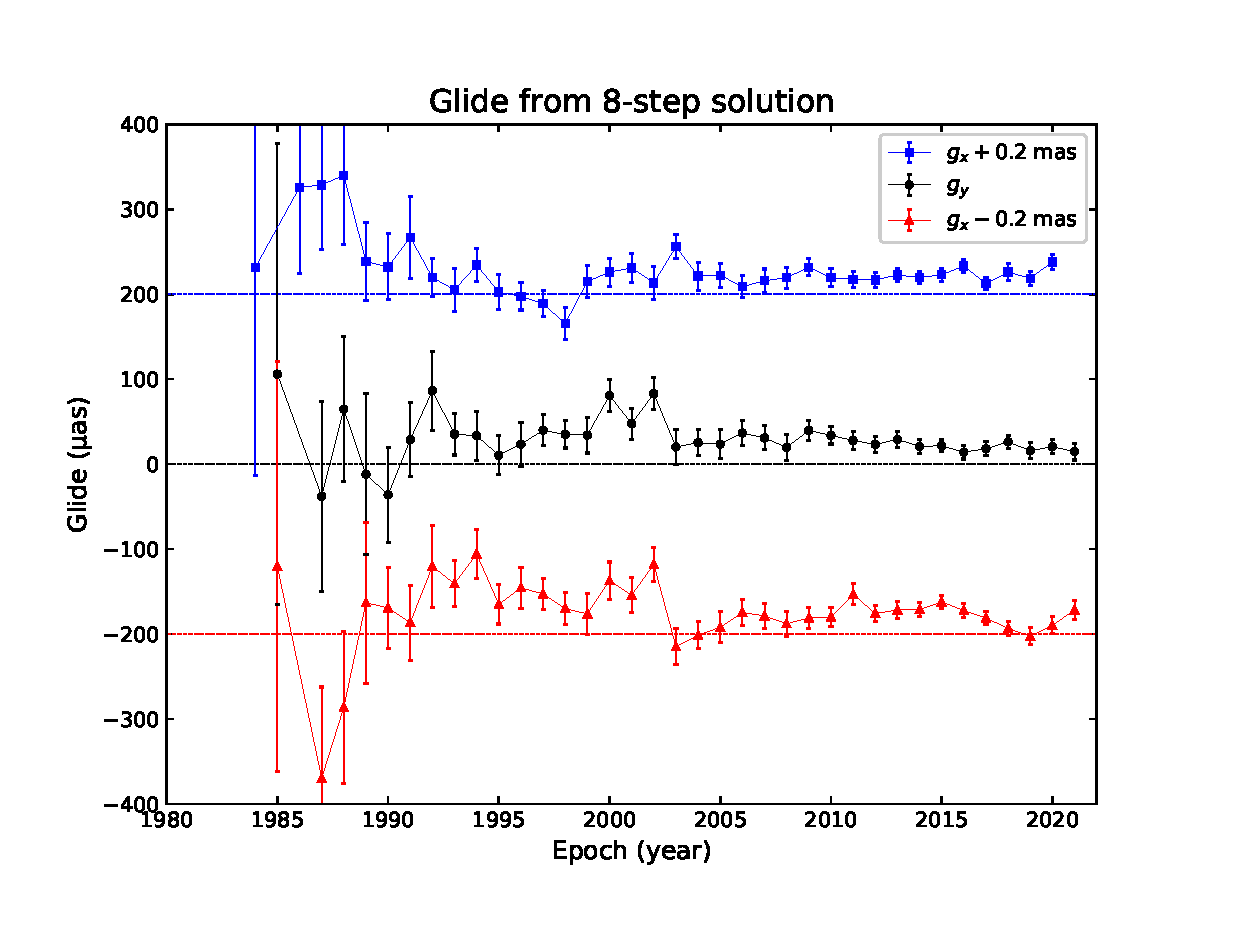
\includegraphics[width=75mm]{figs/glide-from-yearly-ts-nju-8step} \\
   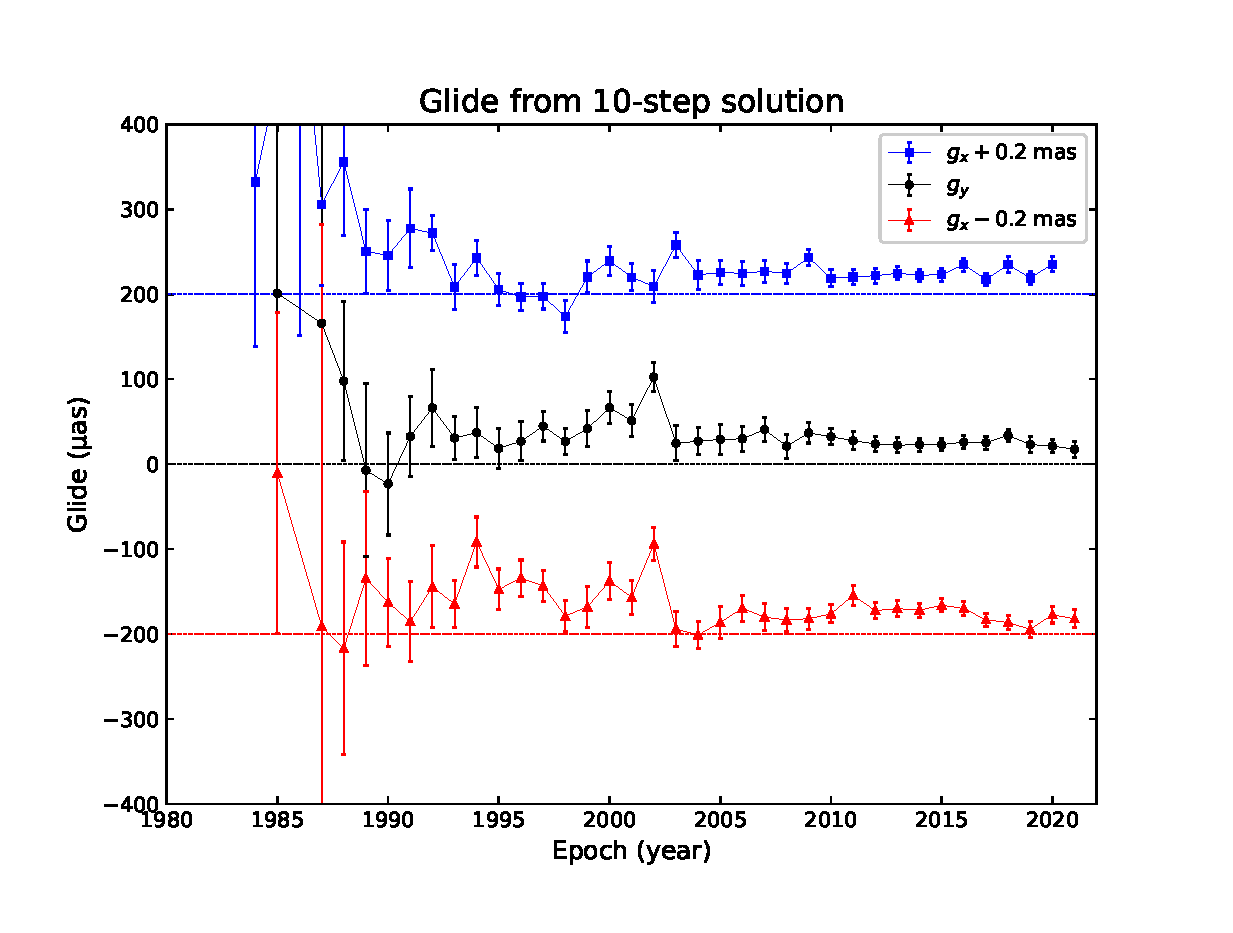
\includegraphics[width=75mm]{figs/glide-from-yearly-ts-nju-10step} 
   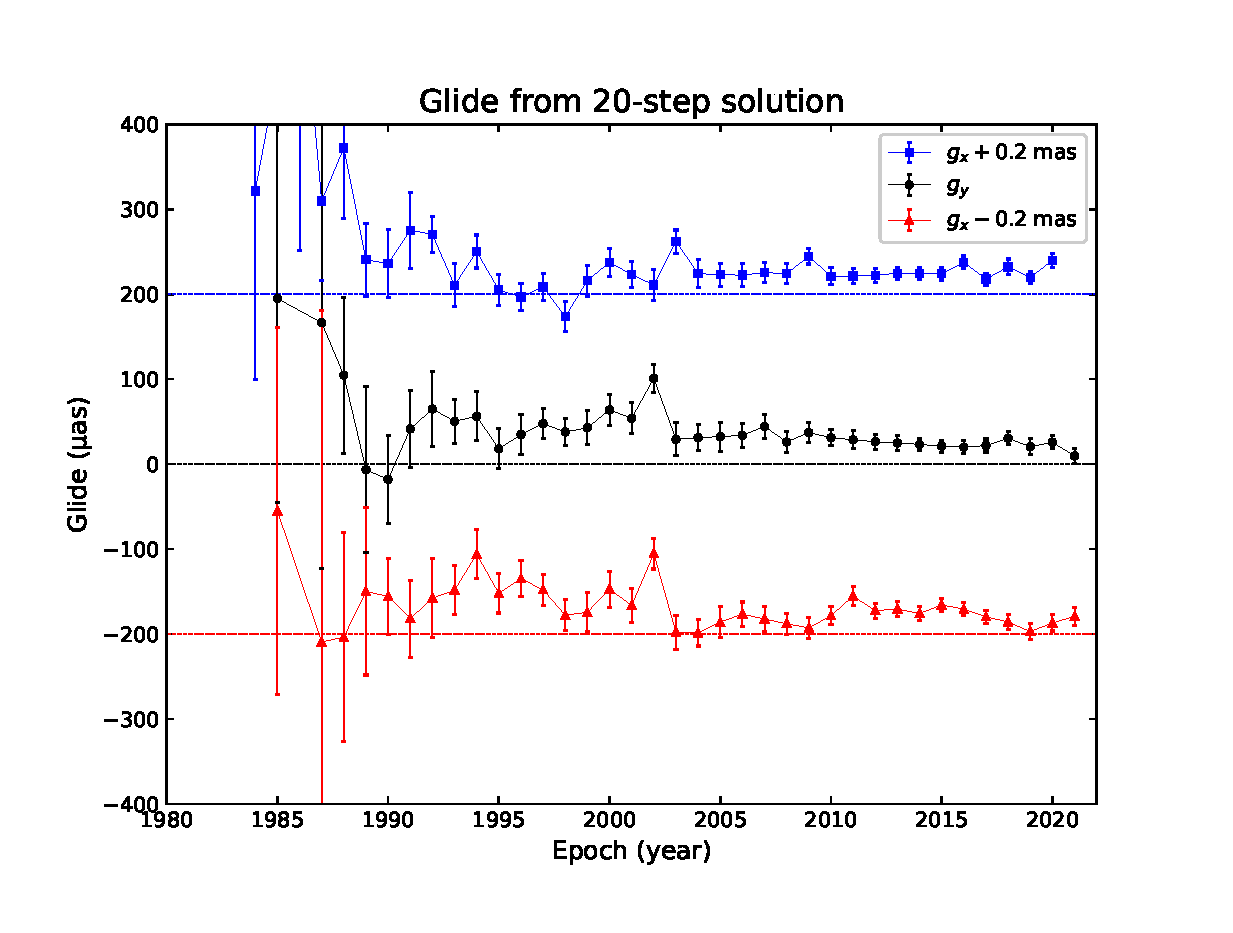
\includegraphics[width=75mm]{figs/glide-from-yearly-ts-nju-20step}  
   \caption[]{\label{fig:glide-plot} %
   Rotation parameters of the yearly CRFs wrt. the ICRF3 S/X-band frame based on the ICRF3 defining sources.
   }
 \end{figure*}
% ===========================================================================
%% Have "floats" such as figures between blank lines to make them float



%% In this file every sentence starts on a new line for better
%% readability, easier change, better synchronization in
%% shared-access systems such as svn, easier use of (mg)diff.
%% This is automatically formatted by emacs in the setup I use,
%% specified in my ~/.emacs shown in "Recipes for linux/unix"
%% on my website.


%\subsection{Method}
%%%%%%%%%%%%%%%%%%%%
% We solved the statistical equilibrium and radiative transfer equations
% for all relevant levels and frequencies in \MgI\ and \MgII\ for
% various models of the solar atmosphere, including the standard one
% formulated in the monumental articles by Vernazza et al.\
% (\citeyearads{1973ApJ...184..605V}, % VALI
% \citeyearads{1976ApJS...30....1V}, % VALII
% \citeyearads{1981ApJS...45..635V}). % VALIII
%% Example same-authors multiple citation list

%    \begin{table}
%        \centering
%        \caption{
%        Orientation offsets with referred to the ICRF3 S/X-band frame.
%        }
%        \begin{tabular}{ccccc}
%            \hline \noalign{\smallskip}
%            & $N_{\rm sou,def}$ & $R_X$ & $R_Y$ & $R_Z$  \\
%            &  &$\mathrm{\mu as}$ & $\mathrm{\mu as}$ & $\mathrm{\mu as}$  \\
%            \noalign{\smallskip}
%            \hline
%            \noalign{\smallskip}
%            ICRF2       & 296  & $ -10$  $\pm$ 7 & $ +20$  $\pm$  8 & $  -1$  $\pm$  7 \\
%            ICRF3-K     & 193  & $ -10 \pm 10$   & $ -9 \pm  11$ & $ -5$  $\pm$  7 \\
%            ICRF3-X/Ka  & 176  & $ -28$  $\pm$ 26 & $ -25$  $\pm$ 27 & $  -52$  $\pm$ 19 \\
%            \noalign{\smallskip}
%            \hline
%        % OPA2019a & 4380 & 2920 & $ +28$  $\pm$  2 & $ -50$  $\pm$  2 & $  -1$  $\pm$  1 \\
%        \end{tabular}
%    \end{table}
%
%    \begin{table}
%        \centering
%        \caption{
%        Orientation offsets with referred to the ICRF3 S/X-band frame from bootstrap sampling.
%        }
%        \begin{tabular}{cccccc}
%            \hline \noalign{\smallskip}
%            & $N_{\rm com}$ & $N_{\rm used}$ & $R_X$ & $R_Y$ & $R_Z$  \\
%            &  &  & $\mathrm{\mu as}$ & $\mathrm{\mu as}$ & $\mathrm{\mu as}$  \\
%            \noalign{\smallskip}
%            \hline
%            \noalign{\smallskip}
%            ICRF2       & 3410 & 2275 & $ -19$  $\pm$  6 & $ +22$  $\pm$  5 & $  +0$  $\pm$  4 \\
%            ICRF3-K     & 793  & 530  & $ -21$  $\pm$  8 & $ -18$  $\pm$  8 & $ -11$  $\pm$  6 \\
%            ICRF3-X/Ka  & 638  & 425  & $ -53$  $\pm$ 19 & $  -7$  $\pm$ 19 & $  +6$  $\pm$ 10 \\
%            % OPA2019a    & 4380 & 2920 & $ +28$  $\pm$  2 & $ -50$  $\pm$  2 & $  -1$  $\pm$  1 \\
%            \noalign{\smallskip}
%            \hline
%        \end{tabular}
%    \end{table}

%%%%%%%%%%%%%%%%%%%%%%%%%%%%%%%%%%%%%%%%%%%%%%%%%%%%%%%%%%%%%%%%%%%%%%%%%%%%
%\section{Conclusion} \label{sec:conclusion}
%%%%%%%%%%%%%%%%%%%%%%%%%%%%%%%%%%%%%%%%%%%%%%%%%%%%%%%%%%%%%%%%%%%%%%%%%%%%
% Our computation explained the formation of the enigmatic
% \MgI\,12\,$\mu$m emission features.
% They arise through population depletion by line photon losses and
% population replenishment from the ionic reservoir through highly
% excited levels.
% A Rydberg-channel replenishment flow is realized by
% collisionally-dominated population diffusion via ladder-wise departure
% divergence (see Fig.~\ref{fig:waterfalls} in
% Sect.~\ref{sec:computations}).
%% Note the tilde.  Fig. \ref would generate too much end-of-sentence space
%% and a line break between Fig. and the number is undesirable

%%%%%%%%%%%%%%%%%%%%%%%%%%%%%%%%%%%%%%%%%%%%%%%%%%%%%%%%%%%%%%%%%%%%%%%%%%%%
\begin{acknowledgements}
  % We are indebted to NASA's \href{http://ui.adsabs.harvard.edu}{ADS}
  % for its magnificent literature and bibliography serving which
  % was severely missed by us -- fortunately unknowingly --
  % in pre-internet 1992.
%% us -- fortunately is A&A style; ApJ wants us---unfortunately.
\end{acknowledgements}

%%%%%%%%%%%%%%%%%%%%%%%%%%%%%%%%%%%%%%%%%%%%%%%%%%%%%%%%%%%%%%%%%%%%%%%%%%%%
%% references
\bibliographystyle{aa-note} %% aa.bst but adding links and notes to references
%%\raggedright              %% for latex+dvips, not for pdflatex
\bibliography{example}      %% example.bib = bibtex entries copied from ADS

\end{document}
